\scanpage{121}
une sorte de synthèse géométrico-arithmétique des nombreuses théories cohomologiques dont on dispose\deleted{\unsure{rait}} à présent pour les variétés algébri\deleted{\unsure{qu}}ques,\deleted{de toutes dimensions,}et des représentations linéaires de groupes de \rlap{\deleted{g}}Galois arithmétiques auxquelles ces théories donnent naissance\deleted{\unsure{s}}.

5) \uline{Solution du problème d'introduction d'une} $\handwritten{\lambda}$-\uline{structure} (correspondant à la notion de puissance extérieure) \uline{dans l'anneau} $K^\bullet(X)$\handwritten{(}dit ``de Grothendieck''\handwritten{)}d'un espace topologique localement annelé (par exemple une variété analytique, ou\deleted{\unsure{nd|md}} différe\rlap{\deleted{\unsure{t}}}nti\rlap{\deleted{b}}a\rlap{\deleted{\unsure{a}}}ble, ou un schéma)\handwritten{,} construit à l'aide de la catégorie des complexes ``parfaits'' sur $X$. Ce problème était signalé comme le plus important problème \mbox{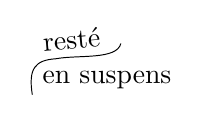
\begin{tikzpicture}[x=1em,y=1em,baseline=(b.base)]
\node[anchor=base west,inner sep=0] (b) at (0,0) {en suspens};
\node[anchor=base west,inner sep=0,rotate=5] at (.05,1.15) {\inserted{\handwritten{resté}}};
\draw[line width=.35pt] (-.35,-.4) .. controls (-.5,.55) and (-.25,.85) .. (.5,.9) .. controls (1.3,1.05) and (2.7,.85) .. (2.85,1.45);
\end{tikzpicture}} dans le Séminaire de Géomé\rlap{\deleted{y}}\handwritten{t}rie Algébrique de l'IHES 1966/67, sur le théorème de Riemann-Roch. La nécessité de travailler avec le $K^\bullet(X)$ défini en termes de \uline{complexes} parfaits, plutôt que de \uline{fibrés} vectoriels seulement, est \unsure{imposé|imposée} par des \deleted{nécess} impératifs techniques irrécusables, qui finiront certainement par s'imposer aussi en dehors de la \rlap{\deleted{\unsure{G}}}\handwritten{g}éométrie algébrique. La solution de Deligne, comme prévu, passe par l'intermédiaire d'une construction de \deleted{puis} foncteurs puissances extérieures dans la catégorie dérivée $D(X)$ (catégorie de\deleted{s} complexes de modules \mbox{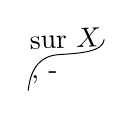
\begin{tikzpicture}[x=1em,y=1em,baseline=(b.base)]
\node[anchor=base west,inner sep=0] (b) at (0,0) {, -};
\node[anchor=base west,inner sep=0,rotate=2] at (-.05,1.05) {\inserted{\handwritten{sur $X$}}};
\draw[line width=.35pt] (-.1,-.45) .. controls (.0,.4) and (.35,.8) .. (1.0,.85) .. controls (1.8,.9) and (2.6,.95) .. (2.65,1.4);
\end{tikzpicture}} en fait, il faut se borner ici aux complexes de \uline{chaines}), en utilisant la théorie de \mbox{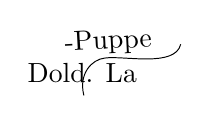
\begin{tikzpicture}[x=1em,y=1em,baseline=(b.base)]
\node[anchor=base west,inner sep=0] (b) at (0,0) {Dold. La};
\node[anchor=base west,inner sep=0,rotate=3] at (1.35,1.15) {\inserted{\handwritten{-Puppe}}};
\draw[line width=.35pt] (2.05,-.45) .. controls (1.85,.35) and (2.35,.85) .. (2.8,.9) .. controls (3.5,1.0) and (5.35,.55) .. (5.55,1.4);
\end{tikzpicture}} difficulté sérieuse consistait à prouver que ces opérations dans $K^\bullet(X)$ satisfont aux propriétés algébriques habituelles, permettant d'exprimer par exemple $\handwritten{\lambda}^i(xy)$ comme polynôme universel à coéfficients entiers en les $\handwritten{\lambda}^j(x),\handwritten{\lambda}^k(y)$. Deligne procède par une voie très ingénieuse, en déterminant d'abord la structure d\unsure{\rlap{u}a|\rlap{a}u} $\handwritten{\lambda}$-anneau de toutes les ``op\rlap{\deleted{\unsure{a}}}érations tensorielles universelles'' qu'on peut effectuer sur des fibrés vectoriels. \rlap{\deleted{\unsure{S|E}}}Il n'a écrit sa théorie que lorsqu'on travaille au dessus d'un corps de base \deleted{\unsure{finis}}\handwritten{(}de caractéristique arbitraire\handwritten{)}. \deleted{Le cas de la caractéristique}
% archive sheet number: 120
